\documentclass[a4paper,11pt]{article}
\usepackage[utf8]{inputenc}

\usepackage{times} % Police de caractères
\usepackage[french]{babel}
\usepackage[top=1.5cm, bottom=1.5cm, left=1.5cm, right=1.5cm]{geometry}

\usepackage{tikz}
\usepackage{graphicx}

\usepackage{algorithm}
\usepackage{algorithmic}

\date{\today}
\title{Projet C - Le Voyageur de commerce}
\author{Alice PELLET -- MARY \& Pierre MACHEREL}

\tikzstyle{vertex}=[circle,fill=black!25,minimum size=20pt,inner sep=0pt]
\tikzstyle{selected vertex} = [vertex, fill=red!24]
\tikzstyle{edge} = [draw,thick,-]
\tikzstyle{weight} = [font=\small]
\tikzstyle{selected edge} = [draw,line width=5pt,-,red!50]
\tikzstyle{cycle} = [draw,line width=5pt,-,black!20]
\tikzstyle{cheminarbre} = [draw,thick,blue]
\tikzstyle{ignored edge} = [draw,line width=5pt,-,black!20]

\begin{document}

\maketitle
\tableofcontents

\section*{Introduction} %Alice

L'objectif de ce projet en binôme de 6 semaines était d'écrire un programme permettant d'approcher le problème du voyageur de commerce. Pour ce faire, nous avons choisi et implémenté différentes structure de données permettant d'enregistrer un grand nombre de données, ou bien de représenter un graphe.\\
Le problème du voyageur de commerce se pose de la façon suivante : on dispose d'une liste de ville qu'un voyageur de commerce voudrait parcourir en minimisant la distance du chemin. Il essaye donc de trouver un chemin minimal passant par toutes les villes et qui revient à son point de départ. Ce problème est un exemple classique de problème NP-Complet : on ne connait pas d'algorithme permettant de le résoudre rapidement (en temps polynomial).\\
Nous avons implémenté un programme basé sur l'algorithme de Prim. Cet algorithme ne donne pas le résultat optimal du voyageur de commerce mais a l'avantage d'avoir une complexité polynomiale.

\section{Structures de données}
Notre programme fait appel à quatre structures de données principales : \textsf{Ville}, \textsf{element\_liste*}, \textsf{Matrice} et \textsf{Tas} qui permettent respectivement de représenter une ville avec ses coordonnées, un arbre, un graphe complet et un ensemble d'arêtes.
Chaque structure présente des avantages (accès à une information en temps constant, recherche d'un minimum dans un ensemble, etc) et des inconvénients (difficulté d'insertion, place en mémoire ...).\\
Pour les structures de données utilisées dans plusieurs fichier, nous avons écrits des fonctions d'accès qui permettent de modifier les structures sans avoir à changer les programmes si on garde le même nom pour les fonctions d'accès.

\subsection{Villes}

Dans l'algorithme, les villes sont représentées par des entiers. On a donc créé un type \textsf{Ville} dans les fichier \emph{structure\_ville}, qui contient le nom de la ville et ses coordonnées. L'ensemble des villes du problème est enregistré dans un tableau de \textsf{Ville}. Cela permet d'associer à chaque ville sa position dans le tableau. Ce tableau est lui même stocké dans la structure \textsf{Matrice} que nous décrirons plus tard.\\
La structure Ville apparait également dans toutes les fonctions liées à la lecture/écriture des villes dans un fichier, ainsi que dans l'interface utilisateur.

\subsection{Arbre couvrant}

L'algorithme que nous avons implémenté nécessite la création d'un arbre couvrant minimal. On le parcourt ensuite pour trouver l'ordre des villes dans le chemin.\\
La structure qui implémente l'arbre couvrant se trouve dans les fichier \emph{structure\_arbre\_couvrant}. 
Pour stocker l'arbre couvrant, on a créé un tableau de type \textsf{element\_liste*}, avec autant de cases qu'il y a de villes dans le graphe, puis dans chaque case i du tableau on stocke sous forme de liste chainée d'entiers les voisins du sommet i dans l'arbre. Comme l'arbre doit être couvrant, tous les sommets sont incidents à au moins une arête, donc on ne gâche pas de place en stockant l'arbre dans un tableau. Une liste chainée présente l'avantage de faciliter l'insertion d'élément, or le nombre de voisin d'un sommet dans l'arbre couvrant minimum n'est pas connu à l'avance.\\
Cet arbre couvrant est également stocké dans la structure Matrice.

\subsection{Matrice} %Alice
Décrite dans les fichier \emph{structure\_matrice}, la structure \textsf{Matrice} contient toutes les informations nécessaires à l'algorithme TSP qui résout le problème du voyageur de commerce :
\begin{itemize}
\renewcommand{\FrenchLabelItem}{\textbullet}
\item Un entier \texttt{nb\_villes} représentant le nombre de villes à parcourir.
\item Une matrice d'adjacence \texttt{graph} qui contient le poids de chaque arête. Les cases (i,j) et (j,i) de la matrice contiennent le poids de l'arête allant du sommet i au sommet j. Une matrice d'adjacence est très volumineuse, mais elle permet d'accéder en temps constant au poids d'une arête.
\item Un tableau d'entiers \texttt{marque} qui sert lors de l'algorithme. Chaque case du tableau représente une ville, qui est marquée si la case contient un 1 et non marquée si elle contient un 0.
\item Un tableau de \textsf{Ville} \texttt{liste\_name} qui permet la conversion entier-ville. Chaque case $i$ du tableau contient la ville associée à l'entier $i$.
\item Un vecteur de listes de sommets \texttt{arbre\_couvrant}qui permet de stocker l'arbre couvrant.
\item Une liste de sommets \texttt{cycle} qui contient le cycle calculé par notre programme.
\item Les coordonnées maximales des villes stockées dans quatre flottants : \texttt{xmin, xmax, ymin, ymax}. Ces données sont nécessaire pour l'affichage graphique.
\end{itemize}

La structure Matrice regroupe l'ensemble des données nécessaire à la résolution du problème du voyageur de commerce et a l'affichage du résultat.
Elle camoufle un pointeur vers une autre structure encapsulée. Cela évite la recopie lorsque elle est donnée en argument dans une fonction. Elle apparait dans les fonctions Prim, TSP ainsi que dans les fonctions auxiliaires à ces 2 fonctions.

\subsection{Arête}
Notre algorithme associe chaque sommet à un entier. Nous avons représenté les arêtes par des couples d'entier $(u, v)$ stocké dans des structures. Une arête $(u, v)$ relie le sommet $u$ au sommet $v$

\subsection{Tas min} %Pierre
L'algorithme Prim appliqué à un graphe $G = (S, A)$ doit trouver $|A|$ fois une arête de poids minimum dans un ensemble donné.
Nous avons donc eu besoin d'une structure de donnée qui permette d'extraire le minimum d'un ensemble avec une faible complexité. Cette structure doit également supporter l'ajout et la suppression d'éléments.
Nous avons choisi d'implémenter cette structure par un tas min.
Un tas min est un arbre ayant les propriétés suivantes :
\begin{itemize}
\item C'est un arbre binaire.
\item Le poids d'un nœud est inférieur à celui de chacun de ses fils. L'élément de poids minimum est donc celui représenté par la racine de l'arbre
\end{itemize}
Le poids d'un nœud est celui de l'élément qu'il décrit.
Chaque élément de l'ensemble à représenter est représenté par un nœud de l'arbre.

Dans le projet, les éléments de l'ensemble sont des arêtes, et leur poids est celui de l'arête dans le graphe. La taille du tas min est donc majorée par le nombre d'arêtes dans le graphe.
Nous avons implémenté le tas min dans une structure \textsf{Tas} contenant :
\begin{itemize}
\renewcommand{\FrenchLabelItem}{\textbullet}
\item Un tableau d’arêtes
\item Une \textsf{Matrice}
\item La taille maximum de l'ensemble que peut représenter l'arbre
\item Le nombre d'éléments stockés dans l'arbre.
\end{itemize}
Le tableau permet de représenter l'arbre du tas min. Il est indexé en partant de 1.
L'indice 1 représente la racine l'arbre (ie l'arête de poids minimum de l'ensemble).
Soit $i$ l'indexe d'un nœud. Ses deux fils (s'ils existent) sont dans les cases d'index $2i$ et $2i +1$ et son père est dans la case d'index $\frac{i}{2}$ (division entière).

Toutes les arêtes qui seront stockées dans le \texttt{Tas} proviendront de la structure \textsf{Matrice}. Avoir accès à celle ci permet au \textsf{Tas} d'accéder aux poids des arêtes.

\section{Définition} %Pierre
Afin de démontrer que l'algorithme que nous avons utilisé retourne une solution dont la longueur n'excède pas deux fois la longueur d'une solution optimale, nous devons introduire un formalisme pour décrire le problème.
\begin{description}
 \item[Graphe non orienté] : Un graphe $G$ est une paire $G = (S, A)$ où :
 \begin{itemize}
 \renewcommand{\FrenchLabelItem}{\textbullet}
  \item S est un ensemble de sommets
  \item A un ensemble d'arêtes qui sont des paire de sommets. Chaque arête relie deux sommet et est pondérée par un poids.
 \end{itemize}
 \item[Chemin] : Un chemin est une suite de sommets $x_1, x_2, \ldots, x_n$ tels que $\left(x_i, x_{i+1}\right) \in A$ avec $i \in \left[1\ldots n-1\right]$
 \item[Graphe connexe] : Un graphe $G$ est connexe si pour toutes paires de sommets $u, v \in G$, il existe un chemin reliant $u$ à $v$.
 \item[Cycle] : Un cycle est un chemin dont tous les sommets sont distincts, sauf les extrémités qui sont égales.
 \item[Cycle hamiltonien] : Un cycle hamiltonien est un cycle qui parcourt l'ensemble des sommets du graphe.
 \item[Arbre] : Un arbre est un un graphe connexe sans cycle
 \item[Arbre binaire] : Un arbre est binaire si chacun de ses nœuds a au plus deux fils.
 \item[Profondeur d'un nœud] : On peut définir un sommet $r$ comme étant la racine de l'arbre. La profondeur d'un élément $s$ dans un arbre est alors le nombre de nœuds qui composent le chemin entre $r$ et $u$.
 \item[Arbre couvrant] : Un arbre $T$ est couvrant sur un graphe $G$ si tous les sommets de $G$ sont dans $T$.
 \item[Arbre couvrant minimum] : Un arbre couvrant est minimum s'il minimise la somme des poids des arêtes qui le composent.
\end{description}

\section{Algorithmes}


L'algorithme que nous avons implémenté pour résoudre le problème du voyageur de commerce est composé de deux fonctions principales, la fonction Prim et une fonction pour parcourir l'arbre couvrant.

\subsection{Prim} %Alice

L'algorithme Prim permet de construire un arbre couvrant minimal à partir d'un graphe. Il prend en entrée une \textsf{Matrice} dont \texttt{arbre\_couvrant} est vide (c'est à dire que le vecteur contient initialement uniquement des listes vides : aucun sommet n'a de voisin). Il la modifie afin que \texttt{arbre\_couvrant} représente un arbre couvrant minimal du graphe.

\subsubsection*{Algo}
\begin{description}
\item[Entrée] : Une Matrice \texttt{M} qui représente le graphe $G = (S, A)$ telle que \texttt{M->arbre\_couvrant} ne contient que des listes vides et \texttt{M->marque} ne contient que des zéros (aucun sommet n'est encore marqué, les sommets marqués sont ceux qui appartiennent à l'arbre couvrant). \texttt{M} doit représenter un graphe complet dont le poids des arêtes respecte l'inégalité triangulaire.
\item[Sortie] : La Matrice \texttt{M} modifiée telle que \texttt{M->marque} ne contient que des 1, c'est à dire que l'arbre couvrant contient tous les sommets. Cet arbre couvrant est minimal.
\end{description}


\textit{Algorithme : } \\
\\
Prim initialise un tas min $T$ qui contiendra des arêtes. La capacité de $T$ est majorée par $|A|$ le nombre d'arêtes du graphe. Le tas min contiendra l'ensemble des arêtes du graphe incidentes à au moins un sommet de l'arbre couvrant en cour de construction.\\
Prim ajoute le sommet 0 à l'arbre (le choix du sommet 0 est arbitraire, on pourrait prendre n'importe lequel).\\
Prim ajoute a $T$ toutes les arêtes du graphe partant de zéro.\\
\\
Tant que toutes les arêtes ne sont pas marquées :
Prim extrait l'arête de poids minimum de $T$ jusqu'à obtenir une arête dont un seul des deux sommets est marqué (c'est fait par la fonction \texttt{trouver\_bonne\_arete} : elle vérifie qu'au moins une des extrémités n'est pas déjà marquée. Puisque les seules arêtes qui sont ajoutées à $T$ sont celles qui ont un sommet marqué, on est assuré que l'arête répond au critère).\\
Prim ajoute cette arête et le sommet non marqué à l'arbre.\\
Puis Prim marque ce sommet et ajoute à $T$ les arêtes partant du sommet qu'il vient d'ajouter et se terminant par un sommet qui n'est pas déjà dans l'arbre.\\
\\
A la fin de cette boucle, tous les sommets ont été marqué et \texttt{M->arbre\_couvrant} contient un arbre couvrant de poids minimal.\\

\begin{algorithm}
\caption{Prim}
\begin{algorithmic}[1]

\STATE Initialiser un tas min de taille $|A|$
\STATE Ajouter le sommet 0 à l'arbre.
\STATE Ajouter au tas toutes les arêtes partant de 0.
\WHILE {l'arbre ne contient pas tous les sommets}
\WHILE {l'arête extraite a ses 2 sommets déjà dans l'arbre}
\STATE Extraire une autre arête.
\ENDWHILE
\STATE Ajouter l'arête extraite à l'arbre.
\STATE Ajouter les sommets de l'arête à l'arbre (un des sommets est déjà dans l'arbre, l'autre non)
\STATE Ajouter les arêtes incidentes à un unique sommet de l'arbre
\ENDWHILE
\STATE Retourner l'arbre.

\end{algorithmic}
\end{algorithm}

\subsubsection*{Complexité}

Soit $n=|S|$ le nombre de sommets du graphe.
L'algorithme utilise un tas min pour extraire l'arête de poids minimal, l'ajout et l'extraction d'un élément dans un tas min se font en $O(log(\frac{n^2}{2}))$, car le graphe est complet, donc $\frac{n(n-1)}{2} = |A|$\\
\\
L'essentiel de la complexité de l'algorithme réside dans les 2 boucles while. Le reste est en $O(n*log(n))$, qui correspond à l'ajout des $n-1$ arêtes dans le tas min (l'ajout d'une arête dans le tas min est en $O(log(n^2)) = O(log(n))$ puisqu'il y a au plus $(n^2)/2$ arêtes dans le tas.\\
\\
On peut aussi remarquer que chaque arête ne peut être ajoutée qu'une fois au tas, donc on peut extraire au maximum $(n^2)/2$ arêtes du tas sur le total de l'algorithme. Au total sur tout l'algorithme, la seconde boucle while fera donc au plus $(n^2)/2$ extractions en $O(log(n))$, donc sa complexité est en $(n^2*log(n))$\\
Enfin, la première boucle while va être parcourue $n$ fois au cours de l'algorithme puisqu'on ajoute exactement un sommet à l'arbre à chaque fois. Et chaque passage a une complexité en $O(log(n)*n)$ pour l'ajout des arêtes au tas min (il y a au plus n arêtes à ajouter). L'ajout d'un sommet et d'une arête à l'arbre se fait en temps constant. Au total cette boucle a donc une complexité en $O(n^2*log(n))$.\\
\\
La complexité totale de l'algorithme est donc en $O(n^2*log(n)+n^2*log(n)+log(n))$, c'est à dire en $O(n^2*log(n))$.


\subsection{Parcourt de l'arbre} %Alice

Après avoir créé un arbre couvrant minimal, l'algorithme TSP que nous avons implémenté a besoin de le parcourir. Pour cela nous avons écrit une fonction \texttt{parcourir\_arbre} dans le fichier \textit{structure\_arbre\_couvrant}.

\subsubsection*{Algo}
Cette fonction écrit le chemin effectué pour parcourir l'arbre dans un fichier donné en entrée. Elle n'écrit chaque nœud qu'une fois. L'idée est de partir d'un nœud, de parcourir récursivement une branche partant de ce nœud, puis de revenir au nœud, de parcourir une autre branche qui en part etc, jusqu'à ce qu'il n'y ait plus de branche non parcourue.

\begin{description}
\item[Entrée] : Une \textsf{Matrice} \texttt{M}, avec \texttt{M->arbre\_couvrant} qui contient l'arbre couvrant calculé par l'algorithme Prim, et un fichier, dans lequel la fonction va écrire le chemin lorsque l'on parcourt l'arbre.
\item[Sortie] : L'algorithme a écrit le chemin du parcourt dans le fichier, et a stocké le parcourt sous forme de liste dans \texttt{M->cycle}.\\
\end{description}

\begin{algorithm}
\caption{parcourt\_arbre\_couvrant}
\begin{algorithmic}[1]

\STATE Partir du sommet 0.
\STATE Écrire 0 dans le fichier.
\STATE Ajouter 0 à la liste des sommet de \texttt{M->cycle}.
\WHILE {la liste des voisins de 0 dans \texttt{M->arbre\_couvrant} est non vide}
\STATE Prendre le premier sommet i de cette liste et le retirer des voisins de 0
\STATE Retirer 0 des voisins du sommet i choisi
\STATE Recommencer au début de l'algorithme en prenant le sommet i au lieu du sommet 0
\ENDWHILE

\end{algorithmic}
\end{algorithm}

\subsubsection*{Complexité}
On parcourt chaque arête au plus 2 fois, dans un sens et dans l'autre. Or un arbre couvrant à $n$ sommets possède $n-1$ arêtes, donc la complexité de l'algorithme est en $O(n)$.

\subsection{TSP}

L'algorithme TSP enfin fait appel aux 2 algorithmes précédents pour calculer un chemin permettant de parcourir toutes les villes sans faire un chemin trop long (on montrera plus loin que notre chemin est au plus 2 fois plus long que le chemin optimal pour parcourir toutes les villes).

\subsubsection*{Algo}
La fonction est assez simple une fois qu'on a les deux fonctions précédentes.
\begin{description}
\item[Entrée] : Une matrice \texttt{M} et un fichier, dans lequel la fonction va écrire le chemin parcouru.
\item[Sortie] : L'algorithme a écrit le chemin du parcourt dans le fichier.\\
\end{description}

\begin{algorithm}
\caption{TSP}
\begin{algorithmic}[1]

\STATE Calculer l'arbre couvrant minimal à partir de la matrice.
\STATE Parcourir l'arbre couvrant.

\end{algorithmic}
\end{algorithm}

\subsubsection*{Complexité}
On a vu que des 2 fonctions précédentes, la première est la plus coûteuse.
La complexité totale de l'algorithme TSP est donc la même que celle de Prim, à savoir $O(n^2*log(n))$.

\subsection{Primitives tas min} %Pierre
La structure \texttt{Tas} supporte 3 primitives :
\begin{itemize}
\item \texttt{extraire\_min} : permet de supprimer et de renvoyer l’élément de poids minimum du tas.
\item \texttt{actualise\_tas} : utilisé uniquement par \texttt{extraire\_min}, cette primitive permet de restaurer les propriétés d'un tas min après la suppressions d'un élément.
\item \texttt{entasser\_element} : permet d'ajouter un élément au tas.
\end{itemize}
\subsubsection*{extraire\_min}
\begin{description}
\item[Entrée] : un \textsf{Tas} $T$ non vide ayant les propriétés du tas min.
\item[Sortie] : un élément $a \in T$ de poids minimum. l'élément de $a$ à été supprimé de $T$, et $T$ a les propriétés d'un tas min.
\end{description}
\paragraph*{Algo}
\texttt{extraire\_min} retourne la racine de $T$. Il faut ensuite supprimer cette racine. Pour ce faire, on écrase la racine par une des feuilles de $T$. Pour finir, il faut restaurer les propriétés du tas min avec la fonction \texttt{actualise\_tas}, car le poids de la feuille déplacée est supérieur à un de ses deux nouveaux fils.
\paragraph*{Complexité}
La complexité de \texttt{extraire\_min} est la même que celle de \texttt{actualise\_tas}
\subsubsection*{actualise\_tas}
\begin{description}
\item[Entrée] : un \textsf{Tas} $T$ non vide et l'indice $i$ à partir du quel actualiser $T$.
\item[Sortie] : le \textsf{Tas} $T$ modifié pour respecter les propriétés du tas min.
\end{description}
\paragraph*{Algo}
Initialement, les sous-arbres dont les racines sont les fils de l'élément $i$ ont les propriétés du tas min. En revanche, il n'y a pas d'information entre le poids de $i$ et le poids de ses fils. L'algorithme va comparer le poids de $i$ avec celui de ses fils et échanger de place $i$ avec son fils de poids minimal, puis répéter l'opération jusqu'à atteindre une feuille ou bien que $T$ ait retrouvé ses propriétés de tas min.\\
Les fonctions $fils\_gauche(i)$ et $fils\_droit(i)$ renvoient les indices des fils de $i$.
\begin{algorithm}
\caption{actualise\_tas}
\begin{algorithmic}[1]
\IF {$poids(fils\_gauche(i)) < poids(fils\_droit(i))$}
\STATE $fils\_min \leftarrow fils\_gauche(i)$
\ELSE
\STATE $fils\_min \leftarrow fils\_droit(i)$
\ENDIF
\IF {$poids(fils\_min(i)) < poids(i)$}
\STATE $Echanger(fils\_min, i)$
\IF {$not Feuille(fils\_min)$}
\STATE $acutalise\_tas(T, fils\_min)$
\ENDIF
\ENDIF
\end{algorithmic}
\end{algorithm}
\paragraph*{Complexité}
Chaque instruction de \texttt{actualise\_tas} s'exécute au plus une fois par appel. Dans le pire des cas, la fonction engendre des appels récursifs jusqu'à atteindre une feuille (ligne 8). La complexité de \texttt{actualise\_tas} est donc en $\mathcal{O}(ln(T.taille\_tas\_courant))$
\subsubsection*{entasser\_element}
\begin{description}
\item[Entrée] :  Un \textsf{Tas} $T$ ayant les propriétés du tas min et un élément $a$.
\item[Sortie] :  $T$ dans lequel on a inséré $a$. $T$ conserve ses propriétés de tas min.
\end{description}
\texttt{entasser\_element} insert $a$ en tant que feuille de l'arbre $T$, puis le fait remonter tant que nécessaire pour récupérer les propriétés du tas min.
La fonction $parent(i)$ renvoient l'indice du père de $i$.
\paragraph*{Algo}
\begin{algorithm}
\caption{entasser\_element}
\begin{algorithmic}[1]
\STATE $T.taille\_tas\_courant \leftarrow T.taille\_tas\_courant + 1$
\STATE $T\left[T.taille\_tas\_courant\right] \leftarrow a$
\STATE $i \leftarrow T.taille\_tas\_courant$
\STATE $j \leftarrow i$
\WHILE {$(j > 1) \&\& (poid(parent(j)) > poid(j))$}
\STATE $Echanger(j, parent(j))$
\STATE $j \leftarrow parent(i)$
\STATE $i \leftarrow j$
\ENDWHILE
\end{algorithmic}
\end{algorithm}
\paragraph*{Complexité}
Dans le pire des cas, le corps de la boucle (ligne 5 à 9) s'exécute jusqu'à ce que $j$ atteigne la racine. La complexité de \texttt{entasser\_element} est donc en $\mathcal{O}(ln(T.taille\_tas\_courant))$


\section{Preuve de 2-approximation} %Pierre
Bien que le problème du voyageur de commerce soit un problème NP-Complet, il existe une solution pour l'approximer si on suppose que ses sommets et le poids des arêtes vérifient l'inégalité triangulaire. Dans ce cas là, l'algorithme que nous avons utilisé est une 2-approximation : la solution retournée par l'algorithme n'excède pas deux fois la longueur d'une solution optimale.

Le poids d'un graph/arbre/cycle est la somme des poids des arêtes qui le compose.
Dans cette section, nous les termes poids et de distance seront équivalents, car dans notre problème, le poids d'une arête $(u,v)$ $(u,v)$ représente la distance séparant les sommets $u$ et $v$.

Le poids d'une solution optimale $c(Opt)$ est borné par le poids d'un arbre couvrant minimal $c(T)$ :
En supprimant une arête de $Opt$, on obtient un arbre couvrant car $Opt$ est un cycle hamiltonien. Par minimalité de $T$, on a donc \begin{equation}
c(T) < c(Opt)
\label{eq1}
\end{equation}

\begin{figure}[!h]
\centering
\begin{tikzpicture}[scale=1, auto,swap]
    % sommet
    \foreach \pos/\name in {{(-1,5)/a}, {(1,3)/b}, {(1,4)/c},{(1,5)/d}, {(2,4)/e}, {(2,2)/f}, {(3,1)/g}, {(4,2)/h}, {(3,3)/i}, {(3,0)/j}, {(1,1)/k}}
        \node[vertex] (\name) at \pos {$\name$};
    % arete
    \foreach \source/ \dest in {a/d, d/e, e/i, i/h, h/g, g/j, j/k, k/f, f/b, b/c, c/a}
        \path[cycle] (\source) -- (\dest);
    \foreach \source/ \dest in {d/e, e/i, i/h, h/g, g/j, j/k, k/f, f/b, b/c, c/a}
        \path[edge] (\source) -- (\dest);
\end{tikzpicture}
\caption{Une solution optimal en gris et un arbre couvrant en noir}
\end{figure}


Soit $C$ le chemin défini comme suit :
Choisir $s \in T$. En partant de $s$, longer les arêtes de $T$ jusqu'à revenir au sommet $s$. Chaque arête de $T$ sera longée deux fois (une fois par côté de l'arête).

\begin{figure}[!h]
\centering
\begin{tikzpicture}[scale=1, auto,swap]
    % sommet
    \foreach \pos/\name in {{(-1,5)/a}, {(1,3)/b}, {(1,4)/c},{(1,5)/d}, {(2,4)/e}, {(2,2)/f}, {(3,1)/g}, {(4,2)/h}, {(3,3)/i}, {(3,0)/j}, {(1,1)/k}}
        \node[vertex] (\name) at \pos {$\name$};
    % arete
    \foreach \source/ \dest in {a/b, b/c, c/d, c/e, b/f, f/k, f/g, g/j, g/h, h/i}
        \path[edge] (\source) -- (\dest);
    \draw[cheminarbre] (a.south west) \foreach \dest in {b.south west, f.west, k.north west, k.west, k.south west, k.south, k.south east, f.south, g.south west, j.west, j.south west, j.south, j.south east, j.east, g.east, h.south east, h.east, h.north east, i.north east, i.north, i.north west, i.west, i.south west, h.west, g.north, f.north east, b.north east, c.south east, e.south, e.south east, e.east, e.north east, e.north, c.north east, d.east, d.north east, d.north, d.north west, d.west, c.west, a.north east}{ -- (\dest)};
\end{tikzpicture}
\caption{Arbre couvrant minimum $T$ en noire et chemin $C$ en bleu}
\end{figure}

\begin{equation}
c(C) = 2c(T)
\label{eq2}
\end{equation}
En combinant (\ref{eq1}) et (\ref{eq2}), on obtient
\begin{equation}
c(C) < 2c(Opt)
\label{eq3}
\end{equation}

Le chemin $C$ n'est pas une solution au problème du voyageur de commerce car des sommets sont parcouru plusieurs fois dans $C$. Cependant, grâce à l'inégalité triangulaire, supprimer un sommet de $C$ n'augmente pas le cout de $C$.
Pour obtenir un cycle à partir de $C = x_1, x_2, \ldots, x_n, x_1$ :
pour chaque sommet $x_i \in C, i\neq1$, conserver uniquement sa première occurrence.

\begin{figure}[!h]
\centering
\begin{tikzpicture}[scale=1, auto,swap]
    % sommet
    \foreach \pos/\name in {{(-1,5)/a}, {(1,3)/b}, {(1,4)/c},{(1,5)/d}, {(2,4)/e}, {(2,2)/f}, {(3,1)/g}, {(4,2)/h}, {(3,3)/i}, {(3,0)/j}, {(1,1)/k}}
        \node[vertex] (\name) at \pos {$\name$};
    % arete
        \foreach \source/ \dest in {a/b, b/f, f/k, k/g, g/j, j/h, h/i, i/c, c/e, e/d, d/a}
        \path[edge] (\source) -- (\dest);
\end{tikzpicture}
\caption{Chemin $W$ en noir}
\end{figure}

\section{Graphique} %Pierre
Le programme offre trois possibilités graphiques :
\subsection{affichage de villes}
Cette option (numéro 3 dans le menu) permet d'afficher un très grand nombre de villes sans en calculer une solution au problème du voyageur de commerce. C'est l'affichage à choisir pour visualiser le fichier \textit{FranceTowns.txt} (\ref{fig1}). L'utilisateur peut fermer la fenêtre avec la croix.
\begin{center}
\begin{figure}[htbp]
\begin{center}
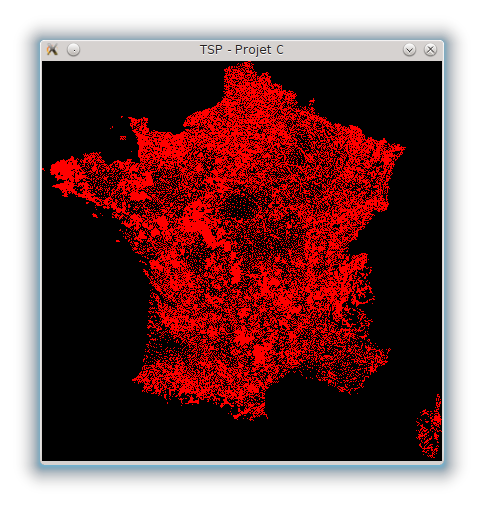
\includegraphics[scale=0.3]{france.png}
\caption{Capture d'écran de l'affichage du fichier FranceTowns.txt}
\label{fig1}
\end{center}
\end{figure}
\end{center}

\subsection{Saisie de villes}
Cette option (numéro 1 $\rightarrow$ 2 dans le menu) permet de cliquer à l'écran pour enregistrer une ville (\ref{fig2}. L'utilisateur ne peut pas supprimer une ville, ni renseigner son nom. Une fois la saisie terminée, l'utilisateur peut fermer la fenêtre avec la croix, la touche esc ou la touche entrée.
\begin{center}
\begin{figure}[htbp]
\begin{center}
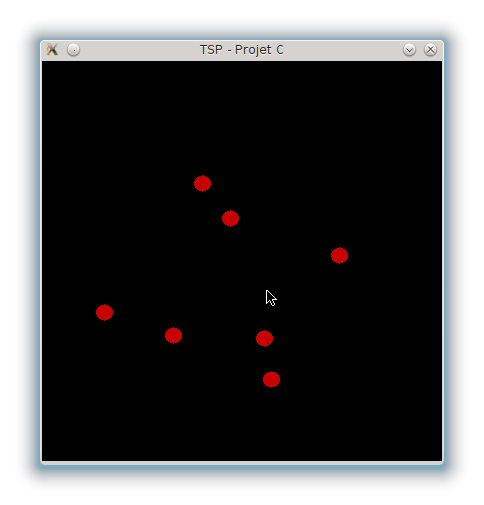
\includegraphics[scale=0.3]{saisie.png}
\caption{Capture d'écran d'une saisie de ville}
\label{fig2}
\end{center}
\end{figure}
\end{center}


\subsection{Affichage d'une solution}
Après que l'utilisateur a généré un fichier ou une solution à un problème, le programme lui propose de visualiser la solution générée graphiquement.
Les touches suivantes permettent d'activer ou de désactiver certaines parties de l'affichage (\ref{fig3}) :
\begin{itemize}
\item c : la solution calculée par le programme.
\item t : l'arbre couvrant calculé par le programme.
\item s : les disques rouges représentant les villes.
\end{itemize}
L'utilisateur peut fermer la fenêtre avec la croix ou avec la touche esc.
\begin{center}
\begin{figure}[h]
\begin{center}
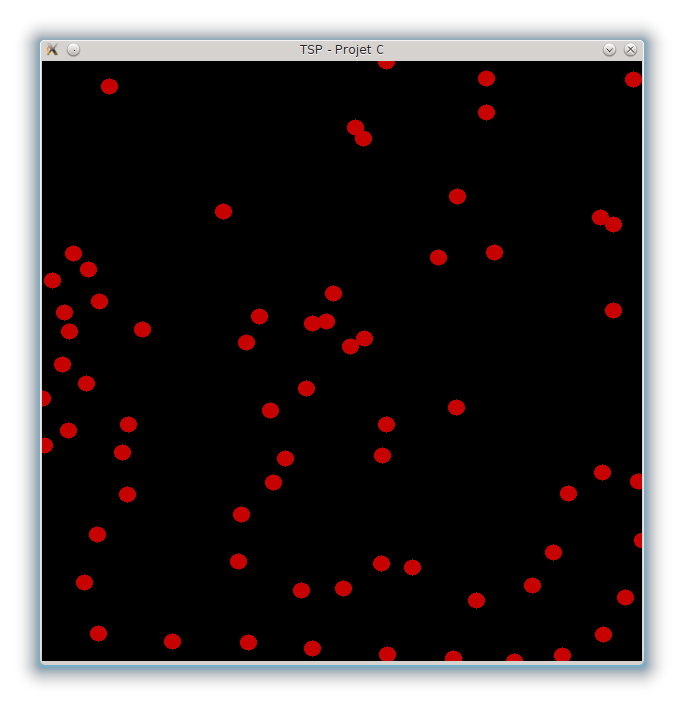
\includegraphics[scale=0.3]{cycleS.png}
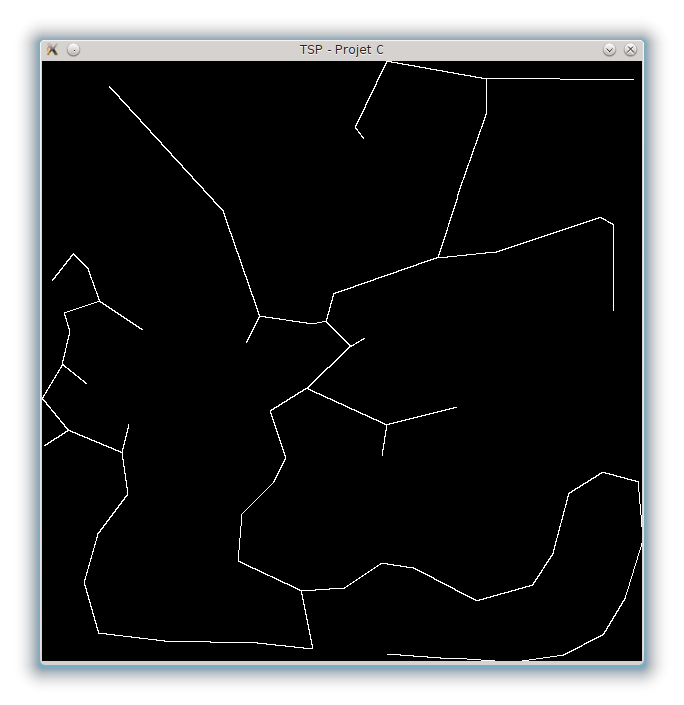
\includegraphics[scale=0.3]{cycleT.png}
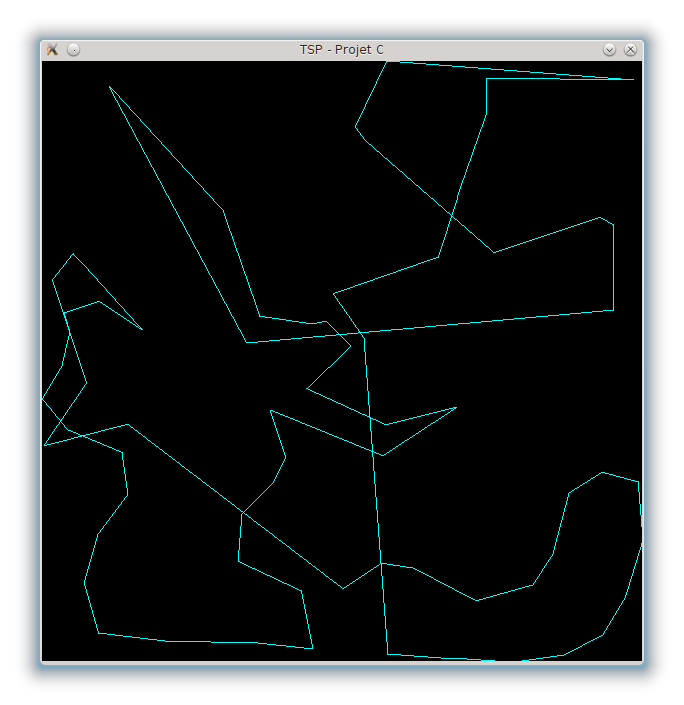
\includegraphics[scale=0.3]{cycleC.png}
\caption{Capture d'écran des différents affichages pour une solution : En rouge les sommets, en bleu le cycle hamiltonien, en blanc l'arbre couvrant minimum}
\label{fig3}
\end{center}
\end{figure}
\end{center}
\section{Utilisation du programme} %Alice

Le programme propose plusieurs choix à l'utilisateur :\\
Un premier menu lui propose :\\
1. De générer la liste des villes par lesquelles il veut faire passer le voyageur de commerce.
A partir de là il choisit de générer sa liste de villes graphiquement ou à partir d'un fichier. S'il décide de la générer graphiquement, une fenêtre s'ouvre et il peut cliquer pour placer ses villes. Une fois la liste de ville complétée, il faut quitter le programme avec la croix, esc ou entrée. L'algorithme affiche ensuite le chemin parcouru par le voyageur de commerce et passant par tous les points.\\
S'il décide de partir d'un fichier, il choisit le fichier qu'il veut utiliser, qui doit être de la forme : \\
\texttt{ville1: 123456; 654321!}\\
\texttt{ville2: 123458; 657521!}\\
Puis il choisit le nombre de villes qu'il veut parcourir, et enfin le nombre de villes qu'il veut rentrer à la main parmi ces villes. Pour les villes qu'il ajoute à la main, le programme cherche dans sa base de donné les coordonnées de la ville. S'il ne la trouve pas, il propose à l'utilisateur de rentrer les coordonnées à la main. L'algorithme écrit ensuite le chemin parcouru dans un fichier dont il demande le nom à l'utilisateur. Il propose également à l'utilisateur de rajouter dans le fichier les villes traversées par le voyageur mais non demandées initialement (il vaut mieux ne pas ajouter les villes traversées si on demande initialement beaucoup de villes car le temps de calcul peut être long).\\
\\
2. D'appliquer l'algorithme Prim à un fichier de villes (toujours de la forme ci dessus), sans possibilité pour l'utilisateur de choisir ses villes.\\
\\
3. D'afficher sur un écran les villes d'un fichier de villes (toujours de la même forme).\\
\\
Si l'utilisateur ne dispose pas de la bibliothèque graphique nécessaire pour afficher les villes, il peut l'installer à l'adresse $\left[\ref{SDL}\right]$ ou bien il peut la désactiver en commentant la première ligne du fichier \textit{main.c}.\\
\\
\textit{Conseils d'utilisation : }\\
Pour des raisons de capacité mémoire des ordinateurs, il vaut mieux ne pas appliquer l'algorithme prim à plus de 10 000 villes.
Lorsque l'on choisit les villes à la main, on peut utiliser le fichier \textit{FranceTowns.txt} qui contient plus de 100 000 villes, mais il vaut mieux ne pas en demander plus de 10 000 pour le parcourt.
Enfin, si on lance l'algorithme prim sur toutes les villes d'un fichier il vaut mieux utiliser le fichier \textit{FranceTownReduced.txt} qui contient moins de villes.


\section{Conclusion} %Alice

Lors de ce projet, nous avons donc codé un programme permettant de donner une approximation du voyageur de commerce en temps polynomial. Nous avons implémenté plusieurs possibilités pour l'utilisateur : rentrer les villes à la main ou les récupérer dans un fichier (ou les 2), mais aussi représenter les villes graphiquement et ajouter les villes traversées mais non demandées initialement.\\
On aurait pu améliorer la complexité spatiale de l'algorithme en évitant de stocker toutes les arêtes dans une matrice. Il aurait fallu pour cela se passer de la structure de tas min qui permet de choisir une arête de poids minimal facilement. De plus, en supprimant la matrice, on ne peut plus utiliser l'algorithme pour des fichiers où l'on donne le poids des arêtes et non pas les coordonnées des points (si le graphe ne vérifie pas l'inégalité triangulaire par exemple). Mais cela aurait permis de lancer l'algorithme sur un plus grand nombre de villes. Actuellement notre algorithme fonctionne (sans l'affichage graphique) pour 10 000 villes sur au moins 2 ordinateurs, mais il n'arrive pas à attribuer assez de mémoire stocker la matrice pour 20 000 villes sur ces 2 mêmes ordinateurs.\\
Le problème du voyageur de commerce peut aussi être approximé grâce à des algorithmes génétiques (sans garantie sur la qualité de l'approximation). 
On génère $x$ cycle hamiltonien, puis on en crée de nouveaux en combinant les solutions précédemment calculées. On conserve ensuite les $x$ meilleures solutions. L'opération peut être répétée un grand nombre de fois pour améliorer le résultat de la meilleure solution calculée.


\section{Références}

Les algorithmes utilisés proviennent de l'énoncé du projet et les fichiers de villes utilisés proviennent de la page perso de Lucie Martinet : \\
$http://perso.ens-lyon.fr/lucie.martinet/enseignements/2012$\_$2013/Projet1/fr/documents$\\
\label{SDL}
$http://www.libsdl.org$, SDL : bibliothèque graphique en c\\
\label{SDLgfx}
$http://www.ferzkopp.net/joomla/content/view/19/14$, SDL\_gfx : surcouche de la SDL\\
Introduction to Algorithms, by Thomas H. Cormen, Charles E. Leiserson, Ronald L. Rivest, and Clifford Stein

\end{document}